\documentclass[11pt,letterpaper]{article}
\special{papersize=8.5in,11in}

\usepackage{fullpage}
\usepackage{amsmath,amssymb,amsthm,dsfont}
\usepackage{xcolor}
\usepackage{float}
\usepackage{tikz}
\usepackage{import}
\usetikzlibrary{shapes.symbols,arrows}

\usetikzlibrary{shapes.symbols,arrows}
\usepackage{enumerate}
\usepackage{enumitem}

\newtheorem{thm}{Theorem}
\newtheorem{pro}[thm]{Proposition}
\newtheorem{lem}[thm]{Lemma}
\newtheorem{cor}[thm]{Corollary}
\newtheorem{defi}[thm]{Definition}

\usepackage[ruled, linesnumbered, noline]{algorithm2e}
\usepackage{listings}
\usepackage{graphicx}
\usepackage{svg}
\usepackage[utf8]{inputenc}
\usepackage[pdftex,pdfpagelabels,bookmarks,hyperindex,hyperfigures]{hyperref}

\usepackage{biblatex}
\addbibresource{dynamic.bib}
\addbibresource{bibase.bib}

\newcommand{\cent}{\gamma}

\newcommand{\ts}{s}
\newcommand{\tf}{\phi}
\newcommand{\try}{\tau}
\newcommand{\dG}{\mathds{G}}
\newcommand{\IN}{\mathds{N}}
\newcommand{\IS}{\mathds{S}}

\newcommand{\In}{\mathrm{In}}
\newcommand{\SM}{{\em SynchMod}$_{\,k}\ $}

% editorial comments in the text or in marginal notes
% 1st argument: initials of the person making the comment,
% 2nd argument: comment to insert
\long\def\ednote#1#2{\par\noindent\framebox{\begin{minipage}{0.99\linewidth}\linespread{.7}\footnotesize #1: #2\end{minipage}}\par}
\newcommand{\edmargin}[2]{\marginpar{\raggedright\linespread{.7}\footnotesize #1: #2}}

\setlength{\parskip}{0.3em}

\title{Synchronization Modulo $k$ in Dynamic Networks}
\author{
	Bernadette Charron-Bost \\
	LIX, Palaiseau, France
% \and
% 	Stephan Merz \\
% 	LORIA, Nancy, France
\and
	Louis Penet de Monterno \\
	LIX, Palaiseau, France
}
\date{\today}

\begin{document}

\maketitle

\ednote{sm}{Use LNCS style and fix affiliations. Also, I should not be an author.}

\begin{abstract}
	We define the mod k—synchronization\edmargin{sm}{mod~$k$-synchronization?} problem as a weakening of the Firing Squad problem,
	where all nodes fire not at the same round, but at rounds that are all equal modulo k.
	We propose an algorithm that achieves mod k—synchronization  in any dynamic network
	with a fixed spanning star. As opposed to the perfect synchronization in
	the Firing Squad problem, mod k—synchronization thus does not require
	any strong connectivity property in the network. 
	Then, we develop our approach for the consensus problem,
        \edmargin{sm}{We use this algorithm as a building block for designing consensus algorithms that tolerate asynchronous starts?}
	and present different consensus algorithms that all tolerate asynchronous starts.
\end{abstract}

% section_intro (do not modify this comment)
\section{Introduction}

Distributed algorithms are often designed in a synchronous computing model, in which computation
	is divided into \emph{communication-closed rounds}:
	any message  sent at some round  can be received only at that round.
In this model it is classically\edmargin{sm}{usually?} assumed that each run of an algorithm is started by all nodes simultaneously, i.e., at the same round,
	or even at round one.
For instance, most of\edmargin{sm}{delete ``of''} synchronous consensus algorithms
	(e.g.,~\cite{PSL80,DS83,ST87}), as well as many distributed algorithms for dynamic networks (e.g.,~\cite{KLO10,KMO11})
	require synchronous starts.

This assumption makes the sequential composition of two distributed algorithms $A;B$
	-- in which each node starts executing $B$ when it has completed the execution of~$A$ --
	quite problematic.
Indeed, nodes start the algorithm~$B$ asynchronously when the algorithm~$A$ terminates asynchronously,
	and the properties of~$B$ are no more guaranteed in this context of asynchronous starts.

This leads to the problem of simulating synchronous starts, classically referred to as
	the {\em firing squad problem}:
\edmargin{sm}{Replace \texttt{\{\textbackslash em ...\}} by \texttt{\textbackslash emph\{...\}} everywhere for better typesetting.}
Each node is  initially  {\em passive} and then becomes {\em active}  at an unpredictable round.
The goal is to guarantee that   the nodes, when all active, eventually synchronize
	by {\em firing} -- i.e., entering a designated state for the first time -- at the same round.

Unfortunately, the impossibility result in~\cite{CBM18} demonstrates that the firing squad problem
	is not solvable without a strong connectivity property of the network, namely, there exists  some positive
	integer~$T$ such that the communication graph within  every period of $T$ consecutive
	rounds is strongly connected and the delay~$T$ is known.
In many situations,  this connectivity property is not guaranteed:
	as an example, in the dynamic graphs corresponding to any system model with benign failures,
	a node  that experiments permanent and complete send omissions
	is  constantly a sink in the  communication graph.

However, with a closer look at many distributed algorithms designed in the round-based model,  we see that
	these algorithms actually  do not require perfectly synchronous starts, and still work under the weaker condition that all the nodes
	start executing the algorithms in rounds with numbers that are equal modulo~$k$, for some positive integer~$k$.
The corresponding synchronization problem, that we call $\mathbf{\mathrm{mod}\,k}$-\emph{synchronization},\edmargin{sm}{Use notation consistently throughout.} is formally specified as follows:
	\begin{description}
	\item[Termination:]   If all nodes are eventually active, then  every node eventually fires.
	\item[$\mathbf{\mathrm{mod}\,k}$-simultaneity:]  If two nodes fire at round~$t$ and $t'$, then $t' \equiv t \mod k$.
	\end{description}

Indeed, let $A$ be an algorithm  organized into regular  \emph{phases} consisting of  a fixed number  $k$ of consecutive rounds:
	the sending and transition functions\edmargin{sm}{The presentation of algorithms has not been described.} of every node at round~$t$ are entirely determined by the value of~$t$ modulo~$k$.
Moreover, assume that $A$ has been proved correct (with respect to some given specification) when all nodes start $A$
	synchronously (at round one) and with any dynamic graph in a family~${\cal G}$ that is stable  under the
	addition of arbitrary finite prefixes.
For instance, the \emph{ThreePhaseCommit} algorithm for non-blocking atomic commitment~\cite{BHG87},
	as well as the consensus algorithms in~\cite{DLS88} or the \emph{LastVoting} algorithm ~\cite{CBS09}
	-- corresponding to the consensus core of \emph{Paxos} -- fulfill all the above requirements
	for phases of length $k=3$ and $k=4$, respectively, and the family ${\cal G}$ of dynamic graphs in which
	there exists an infinite number of ``good'' communication patterns
	(e.g., a sequence of $2k-1$ consecutive communication graphs  in which a majority of nodes is heard by all
	in   each graph).
The use of a $\mathrm{mod}\,k$-synchronization algorithm on the top of\edmargin{sm}{What does ``on [the] top of'' mean?} the algorithm $A$ yields a new algorithm that executes
	exactly like $A$ does, after a finite preliminary period during which every node becomes active and fires.
The above property on the set of dynamic graphs ${\cal G}$ then guarantees this variant of $A$ to be correct with
	asynchronous starts and dynamic graphs in ${\cal G}$.

Another typical example for which perfect synchronization can be weakened to synchronization modulo $k$ is
	the development of the basic \emph{rotating coordinator} strategy in the context of asynchronous starts.
Roughly speaking, this strategy consists in the following: if nodes have unique identifiers in $\{1,\dots,n\}$,
	the coordinator at round~$t$ is the node whose identifier is  $t$ modulo~$n$.
For that, 	 each node~$u$ maintains a local counter $c_u$
	whose current value is the number of rounds where it has been active.
At each round, the  coordinator of $u$ is the  node with the identifier that is equal to the current value of $c_u$ modulo~$n$.
Since there may be only one coordinator per round, such a selection rule requires synchronous starts.
Clearly, with the use of a $\mathrm{mod}\,k$-synchronization\edmargin{sm}{mod~$n$?} algorithm in a preliminary phase and a
	counter for each node that now counts the number of rounds elapsed since the node fired, the above scheme correctly\footnote{%
	With respect to a specification that lets a passive node be  a coordinator.}
	implements the rotating coordinator strategy in the context of asynchronous starts.

% section_model (do not modify this comment)
\section{Preliminaries}\label{sec:model}
 
\subsection{The computational model}
	
We consider a networked system with a {\em fixed} set $V$ of $n$ nodes.
We assume a round-based computational model  in the spirit of the Heard-Of model~\cite{CBS09}, 
	in which point-to-point communications are organized into \emph{synchronized rounds}: 
	each node can send messages  to all nodes and can receive messages sent  by some of the nodes.
Rounds are communication closed in the sense that no node receives messages in round~$t$ that are sent 
	in a round different from~$t$. 
The collection of \emph{possible} communications (which nodes can communicate to which nodes) at each round $t$
	is modelled by a directed graph (digraph, for short) with a set of nodes equal to~$V$.
The digraph at round~$t$ is  denoted $\mathds{G}(t)=(V,E_t)$, and is called the \emph{communication graph at round}~$t$. 
The set of $u$'s incoming neighbors in the digraph $\mathds{G}(t)$ is denoted by $\mathit{In}_u(t)$.

We assume a self-loop at each node in all these digraphs  since every node can communicate with 
	itself instantaneously.	
The sequence of such digraphs~$\mathds{G}=\left (\mathds{G}(t) \right )_{t\in \mathds{N}}$ is called a {\em dynamic graph}~\cite{CFQS11:TVG}. 

In round $t$ ($t = 1, 2 , \ldots $), each node~$ u $ successively
	(a) broadcasts  messages determined by its state at the beginning of round~$t$,
	(b) receives \emph{some} of the messages sent to it,
	and finally (c) undergoes\edmargin{sm}{performs?} an internal transition to a new\edmargin{sm}{successor?} state.
A  \emph{local algorithm} for a node corresponds to a pair of
	a \emph{sending function} that determines the messages to be sent in step~(a)
	and a \emph{transition function} for state updates in step (c).
An \emph{algorithm} for the set of nodes~$V$ is a collection of local algorithms, one per node.

We also introduce the notion of  \emph{start schedules}
	that are collections~$\mathds{S}= \left (s_u \right )_{u \in V}$,
	where each~$s_u$ is  a positive integer or is equal to $\infty$.

	
The execution of the algorithm $ A $  with the dynamic graph $\mathds{G}$ and the start schedule $\mathds{S}$ then proceeds
	as follows:
Each node~$u$ is initially  \emph{passive}. 
If $s_u = \infty$, then  the node~$u$ remains passive forever.
Otherwise, $s_u $ is a positive integer, and $u$ becomes {\em active} 
	at the beginning of round~$s_u$, sets up its local variables.
In  round~$t$ $(t = 1,2\dots)$, a passive  node
	sends only heartbeats, corresponding to  \emph{null} messages,  and  cannot change its state. 	
An active node 	applies its sending function in~$A$ to its current state to generate the message\edmargin{sm}{necessarily the same?} to be sent to all nodes,
	then it receives the messages sent by its incoming neighbors in the directed graph~$\mathds{G}(t)$, and finally 
	applies its transition function ${\cal T}_u$ in~$A$ to its current state and the list of messages it has just received
	(including the null messages from passive nodes), to go to a\edmargin{sm}{compute its?} next state. 
Since each local algorithm is deterministic, an execution of the algorithm~$A$  is entirely determined 
	by the initial state of the network,  the dynamic graph $\mathds{G}$,
	and  the  start schedule~$\mathds{S}$.
	
The states ``passive'' and ``active'' do not refer to any physical notion, and are relative to the algorithm under consideration:
	as an example, if two algorithms $A$ and $B$ are sequentially executed according to the order ``$A$ followed by $B$'',
	then at some round, a node may be active w.r.t. $A$ while it is passive w.r.t. $B$.
In such a situation, the node  is integrally part of the system and can send messages, but  these messages are empty 
	with respect to the semantics of~$B$.
	
\subsection{Network model and start model}

Let us recall the notion of \emph{product} of two graphs $G_1 = (V, E_1)$ and $G_2 = (V, G_2)$, denoted $G_1 \circ G_2$. This notion is defined in \cite{CBM19}.
$G_1 \circ G_2$ has $V$ as its set of nodes, and $(u,v)$ is an edge if there exists $w \in V$ such that $(u,w) \in G_1$ and $(w,v) \in G_2$.
For any dynamic graph $\mathds{G}$ and any integer $t' \geq t \geq 1$, we let $\mathds{G}(t:t') = \mathds{G}(t) \circ \mathds{G}(t+1) \circ \dots \circ \mathds{G}(t')$.
When $t' < t$, $\mathds{G}(t:t')$ is the graph with only a self-loop at each node.
Intuitively, the graph $\mathds{G}(t+1:t')$ contains an edge $(u,v)$ if some information about the state of node $u$ in round $t$ may reach node $v$ in round $t'$.
The set of incoming neighbors of $u$ in $\mathds{G}(t:t')$ is noted as $\mathit{In}_u(t:t')$.
The set $\mathit{In}_u(t:t)$ is simply noted $In_u(t)$.
An \emph{$u \sim v$ path in the interval $[t,t']$}\edmargin{sm}{$\sim$ usually denotes an equivalence relation.} is a finite sequence $u = w_{t-1}, w_t, \cdots, w_{t'} = v$
such that for any $l < t'-t+1$, the edge $(w_{t+l-1},w_{t+l})$ belongs to $E_{t+l}$.
This path is said to be \textit{active} if every node $w_{t''}$ is active in round $t''$ where $t \leq t'' \leq t'$.
There exists a $u \sim v$ path in the interval $[t,t']$ if and only if $v \in \mathit{In}_u(t:t')$.

A \emph{network model} is any non-empty set of dynamic graphs with a permanent self-loop at each node.
We will focus on the specific network models $\mathcal{G}_{k-centered}$ of dynamic graphs~$\mathds{G}$ \emph{centered with delay $k$} verifying: 

$$\exists \cent \in V, \forall t \in \mathds{N}, \forall u \in V, \cent \in \mathit{In}_u(t+1:t+k).$$

The nodes $\cent$ verifying this property are called \textit{$k$-centers}.
There may be several $k$-centers for $\mathds{G}$.
The network class $\mathcal{G}_{k-centered}$ is a super-set of $\mathcal{G}_{1-centered}$, which contains the dynamic graphs containing a fixed spanning star.
Here, $k$ is the parameter of the $\mathrm{mod}\,k$-synchronization problem.
%% sm: redundant with above
% We note $\cent$ one of these $k$-centers.

Similarly, we define a \emph{start model} as a non-empty set of start schedules.
A start schedule $\mathds{S} = (s_u)_{u\in V}$ is \emph{complete} if every $s_u$ is finite, i.e.,
no node is passive forever, yielding the model of complete start schedules.
Synchronous starts correspond to complete start schedules $\mathds{S} = (s_u)_{u\in V}$ with
equal start rounds.	
The property of synchronous starts can be relaxed into \emph{$\mathrm{mod}\,k$-synchronous starts},
where $k$ is any positive integer: for every pair of nodes~$u$ and $v$, it holds that $s_u \equiv s_v \!\mod k$.

% section_algorithm (do not modify this comment)
\section{The algorithm}

We consider some $k > 2$.
In this algorithm, the nodes hold a $level$ variable. When they start, they move from passive state to level 0. They later move to level 1, then to level 2.
Each time a node moves from some level to the next, this constitutes a \emph{level-up} event, whose \emph{strength} is the reached level.
A node fires when it reaches level 2.
The conditional statements \ref{line:level1up} and \ref{line:cond-firing}\edmargin{sm}{at lines ... of Algorithm 1 (and the numbers are wrong). Show the algorithm earlier in the paper.} are executed when the node reaches level 1 and 2 respectively.
The intuition of the algorithm can be summarized by two simple ideas:

Firstly, \textbf{each node keeps track of the most recent strongest level-up.}
Only the strongest level-up events are considered: if some node ``knows'' about a level-up from level 1 to level 2,
it will not record any level-up from level 0 to level 1, nor any level-up from passive state to level 0.
Among the strongest level-up events, the nodes keep track of the age of the most recent one.
For that purpose, they hold two variables $c_u$ and $\mathit{force}_u$.
At any round, node $u$ knows that $c_u$ rounds ago, some node reached a level equal to $\mathit{force}_u$ from the previous level,
and the node does not know any node which reached a level equal to $\mathit{force}_u$ (or higher) in any more recent round.
With lines~\ref{line:force} and \ref{line:min-z-end}, they use at each round the values from their incoming neighbors to update theirs.
The presence of self-loops implies that these lines are always well-defined objects.\edmargin{sm}{the minima and maxima are well-defined}

\begin{figure}[h!]
	\centering
	\caption{case where every node is congruent to 0 in round $t-k$}
	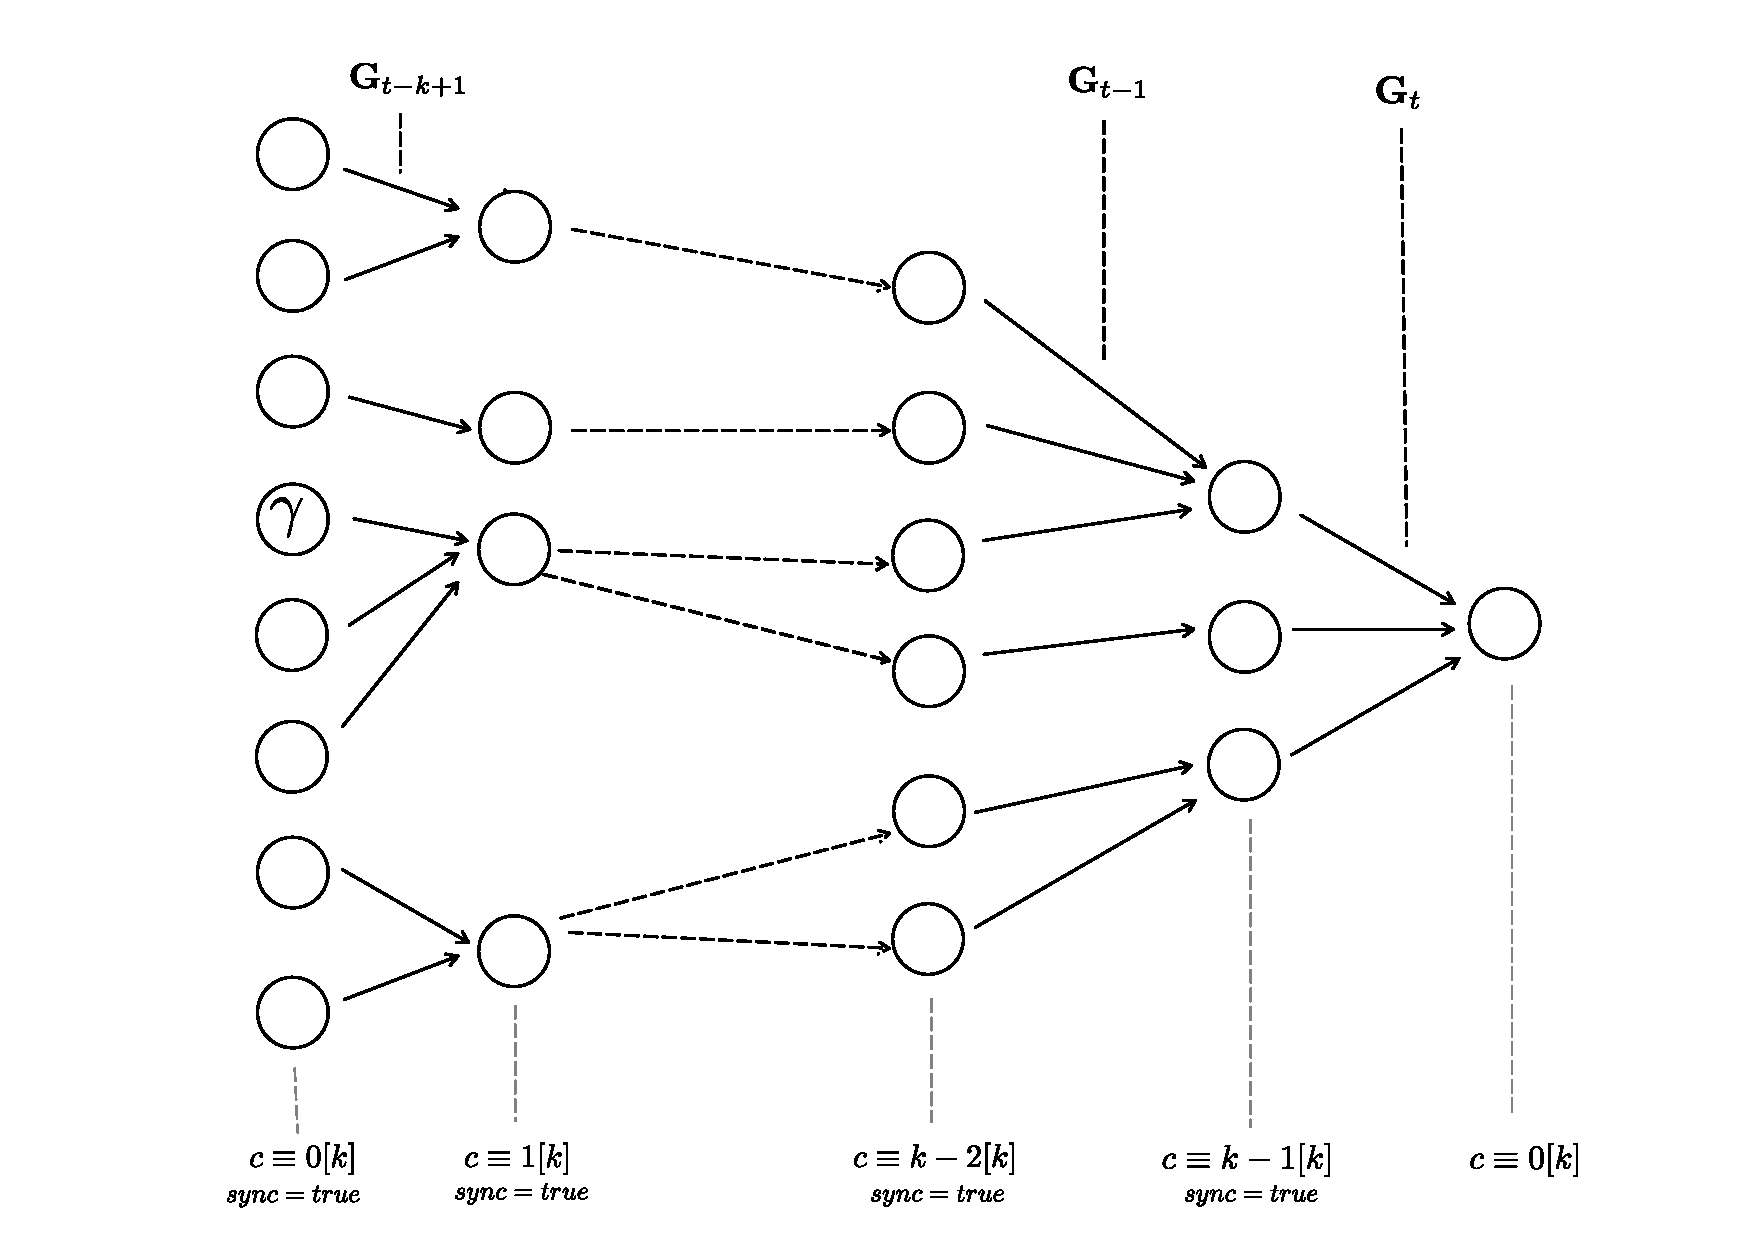
\includegraphics[width=0.7\columnwidth]{illustration-conc-1}
	\label{fig:fig1}
\end{figure}

\begin{figure}[h!]
	\centering
	\caption{case where some node are not congruent to 0 in round $t-k$}
	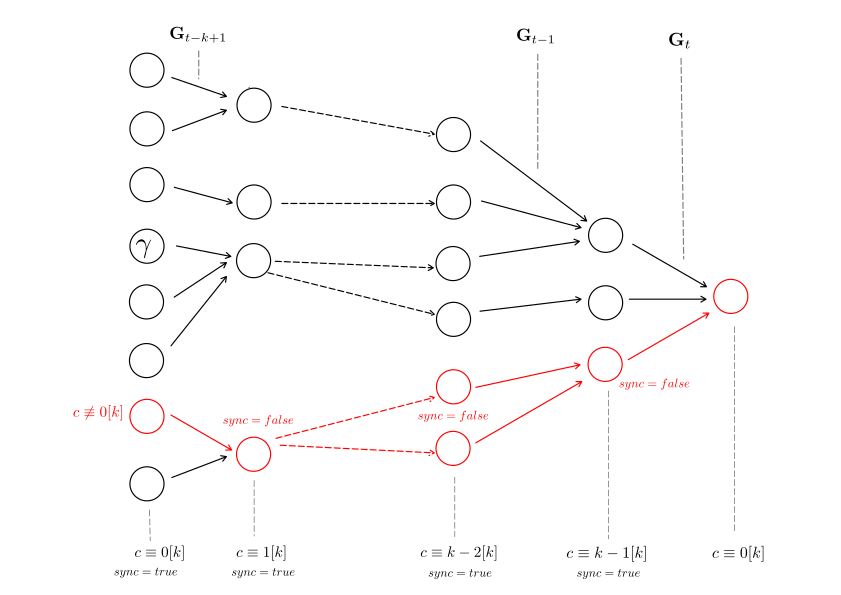
\includegraphics[width=0.7\columnwidth]{illustration-conc-2}
	\label{fig:fig2}
\end{figure}


Secondly, \textbf{a node may level up only if its counter $c_u$ is congruent to 0 and the counter of $\gamma$ was also congruent to 0 $k$ rounds ago.}\edmargin{sm}{Does the node know a fixed $\cent$?}
For that purpose, they use a Boolean variable $\mathit{synch}$.
When the counter of some node $u$ becomes congruent to 0 in some round $t$, it sets its $\mathit{synch}_u$ variable to $\mathit{true}$ in line~\ref{line:conc-true}.
During all subsequent rounds $t+i$, it will check whether the counters of its incoming neighbors are all congruent to its own counter (line~\ref{line:conc-gossip}).
In case they are not, the node will set its $\mathit{synch}_u$ variable to $\mathit{false}$. % (see figure \ref{fig:fig2}). [sm: the reference below is more appropriate]
This $\mathit{false}$ value will disseminate to its outgoing neighbors (also line~\ref{line:conc-gossip}).
If, in round $t+k$, its $synch_u$ variable is still true, node $u$ knows that no non-congruence was detected between round $t$ and round $t+k$.
This means that $\cent$\edmargin{sm}{every center $\cent$?} was congruent with 0 in round $t$.
In that case, a level-up is allowed\edmargin{sm}{will take place?} (see figure \ref{fig:fig1}).
In contrast, if some node $j \in \mathit{In}_u(t+1:t+k)$ is not congruent with 0 in round $t$,
then the line~\ref{line:conc-gossip} guarantees that $\mathit{synch}_u$ will ultimately be $\mathit{false}$ at the beginning of round $t+k$ (see figure \ref{fig:fig2}).
In addition to $\mathit{synch}$, the $\mathit{ready}$ variable makes sure that $\cent$ is already at level 1.
If not, the level-up to level 2 is forbidden.


\begin{algorithm}[hbt!]
	\DontPrintSemicolon
	\textbf{Initialization:} \;
	\Indp
		$c_u \in \mathds{N}$, initially 0 \;
		$\mathit{synch}_u \leftarrow \mathit{false}$ \;
		$\mathit{ready}_u \leftarrow \mathit{false}$ \;
		$\mathit{force}_u \in \{0, 1, 2\}$, initially 0 \;
		$\mathit{level}_u \in \{0, 1, 2\}$, initially 0 \;
	\BlankLine
	\Indm
	\textbf{At each round:} \;
	\Indp
		send $\langle c_u, \mathit{synch}_u, \mathit{force}_u, \mathit{ready}_u \rangle$ to all  \;
		{\small receive incoming messages: let $\mathit{In}^a$ the set of nodes from which a non-null message is received.} \;
		\If{all received messages are non-null}{ \label{line:nonull}
			$\mathit{synch}_u \leftarrow \underset{v \in \mathit{In}^a}{\bigwedge} \mathit{synch}_v \wedge c_v \equiv c_u \mod k$ \; \label{line:conc-gossip}
		}
		\Else{$\mathit{synch}_u \leftarrow \mathit{false}$}
		$\mathit{ready}_u \leftarrow \underset{v \in \mathit{In}^a}{\bigwedge} \mathit{ready}_v $ \; \label{line:ready-gossip} 
		$\mathit{force}_u \leftarrow \underset{v \in \mathit{In}^a}{\max} \mathit{force}_v$ \;\label{line:force}
		$c_u \leftarrow 1+ \underset{\mathit{force}_v = \mathit{force}_u}{\underset{v \in \mathit{In}^a}{\min}} c_v$ \;\label{line:min-z-end} 
		\If{$c_u \equiv 0 \mod k$}{ \label{line:cond-levelup} 
			\If{$\mathit{level}_u = 0 \wedge \mathit{synch}_u$}{ \label{line:level1up}
				$\mathit{level}_u \leftarrow 1$ \; \label{line:level1}
				\If{$\mathit{force}_u < 2$}{
					$\mathit{force}_u \leftarrow 1$ \; \label{line:force2}
					$c_u \leftarrow 0$ \; \label{line:force3}
				}
			}
			\ElseIf{$\mathit{level}_u = 1 \wedge \mathit{ready}_u \wedge \mathit{synch}_u$}{ \label{line:cond-firing}
				$\mathit{level}_u \leftarrow 2$ \tcc*[f]{the node $u$ fires}\; \label{line:level2}
				$\mathit{force}_u \leftarrow 2$ \; \label{line:force5}
				$c_u \leftarrow 0$ \; \label{line:force4}
			}
			$\mathit{synch}_u \leftarrow \mathit{true}$ \; \label{line:conc-true}
			$\mathit{ready}_u \leftarrow \mathit{level}_u > 0$ \; \label{line:init-ready}
		}
	\Indm
\caption{The \SM algorithm} 
\end{algorithm}

\subsection{Notation and preliminary lemmas}
\ednote{sm}{It is considered bad style to start a subsection after several pages of a section.}

In the rest of this section, we fix an execution $\sigma$ of the \SM algorithm associated to a complete activation
schedule~$\mathcal{A}$ and a $k$-centered dynamic graph~$\mathds{G} \in \mathcal{G}_{k-centered}$. 
Let $s^{\max} = \max_{u \in \Pi} s(u) < \infty$ and let~$\cent$ denote some center of~$\mathds{G}$.

We note $c_u(t), \mathit{synch}_u(t), \dots$ the values of the variables $c, \mathit{synch}, \dots$ of node $u$ at the end of round $t$, if $u$ is active in round $t$.
The values $c_u(t), \mathit{synch}_u(t), \dots$\edmargin{sm}{These values?} refer to the initial state if the node $u$ starts in round $t+1$.
We also note $c^{pre}_u(t), \mathit{synch}^{pre}_u(t), \dots$ the values of the $c, \mathit{synch}, \dots$ variables
of node $u$ at the beginning of line~\ref{line:cond-levelup} during round $t$, if $u$ is active in round $t$.
We now prove that this execution verifies both properties of the $\mathrm{mod}\,k$-synchronization problem.
We note $\mathit{In}_u^a(t)$ the subset of nodes in $\mathit{In}_u(t)$ which are active in round $t-1$ in this execution.
Some simple claims are deductible from the transition function.
We consider some node $u \in V$ and some round $t$ in which $u$ is active (i.e., $t \geq s_u$).
\begin{lem} \hfill
	\begin{enumerate}[label=\upshape(\alph*),ref=\thethm (\alph*)]
		\item\label{lem:cl1} $\mathit{level}_u(t+1) \in \{\mathit{level}_u(t), \mathit{level}_u(t)+1\}$
		\item\label{lem:cl2b}$c_u(t) \neq 0 \Rightarrow (\mathit{force}_u(t) = \mathit{force}_u^{pre}(t) \wedge c_u(t) = c_u^{pre}(t))$.
		\item\label{lem:cl2} $c_u(t) \equiv c_u^{pre}(t) \mod k$.
		\item\label{lem:cl3} $\mathit{synch}_u^{pre}(t) \Rightarrow \forall v \in \mathit{In}_u(t), c_v^{pre}(t-1) + 1 \equiv c_u^{pre}(t) \mod k$.
		\item\label{lem:cl4} $c_u^{pre}(t) \not\equiv 1 \mod k \wedge \mathit{synch}_u^{pre}(t) \Rightarrow \forall v \in \mathit{In}_u(t),\, \mathit{synch}_v^{pre}(t-1)$.
		\item\label{lem:cl5} $c_u^{pre}(t) \not\equiv 1 \mod k \wedge \mathit{synch}_u^{pre}(t) \wedge \mathit{ready}_u^{pre}(t) \Rightarrow \forall v \in \mathit{In}_u^a(t),\, \mathit{ready}_v^{pre}(t-1)$.
		\item\label{lem:cl6} $\forall v \in \mathit{In}_u^a(t),\, \mathit{force}_v^{pre}(t-1) \leq \mathit{force}_v(t-1) \leq \mathit{force}_u^{pre}(t) \leq \mathit{force}_u(t)$.
		\item\label{lem:cl7} $\forall v \in \mathit{In}_u^a(t),\, \mathit{force}_v^{pre}(t-1) = \mathit{force}_u^{pre}(t) \Rightarrow c_u^{pre}(t) \leq 1+c_v(t-1) \leq 1+c_v^{pre}(t-1)$.
	\end{enumerate}
\end{lem}
\begin{proof}\edmargin{sm}{These proofs could be removed if you need space.} \mbox{}
	\begin{enumerate}[label=\upshape(\alph*),ref=\thethm (\alph*)]
		\item The value of $\mathit{level}_u(t+1)$ is equal to $\mathit{level}_u(t)$, unless line~\ref{line:level1} or \ref{line:level2} is executed in round $t+1$.
			In that case, $\mathit{level}_u(t+1) = \mathit{level}_u(t)+1$.
		\item The conditional statement starting in line~\ref{line:cond-levelup} either sets $c_u(t)$ to 0 (in line~\ref{line:force3} or \ref{line:force4}),
			or does not modify $c_u(t)$ or $\mathit{force}_u(t)$.
		\item In each case above, the value of $c_u(t)$ is not modified modulo $k$.
		\item Firstly, $c_v^{pre}(t-1)$ is well-defined because $\mathit{In}_u(t) = \mathit{In}_u^a(t)$ (see line~\ref{line:nonull}). 
			Moreover, the set $\{c_v(t-1), v \in \mathit{In}_u(t)\}$ contains integers which are mutually congruent modulo $k$ (see line~\ref{line:conc-gossip}).
			Because of line~\ref{line:min-z-end}, we have $c_v(t-1) + 1 \equiv c_u^{pre}(t) \mod k$.
			Finally, $c_v(t-1) \equiv c_v^{pre}(t-1) \mod k$ always holds.
		\item If $c_u^{pre}(t) \not\equiv 1 \mod k$ and $\mathit{synch}_u^{pre}(t) = \mathit{true}$, then every incoming neighbor of $u$ is active in round $t-1$, because\edmargin{sm}{??} .
			and $v$ verifies $\mathit{synch}_v(t-1) \wedge c_v(t-1) \not\equiv 0 \mod k$ (see line~\ref{line:conc-gossip}).
			Then the conditional statement starting in line~\ref{line:cond-levelup} is not executed by $v$ in round $t-1$.
			Then, from $\mathit{synch}_v(t-1)$, the variable $\mathit{synch}_v^{pre}(t-1)$ is true.
		\item Assume that $c_u(t) \not\equiv 1 \mod k \wedge \mathit{ready}_u^{pre}(t) \wedge \mathit{synch}_u^{pre}(t)$.
			Using the previous proof, every incoming neighbor $v$ is active in round $t-1$ and
			the conditional statement starting in line~\ref{line:cond-levelup} is not executed by $v$ in round $t-1$.
			Finally, by line~\ref{line:ready-gossip}, $v$ verifies $\mathit{ready}_v^{pre}(t-1)$.
		\item This property follows directly from lines \ref{line:force}, \ref{line:force2} and \ref{line:force5}.
		\item If $\mathit{force}_v^{pre}(t) = \mathit{force}_v^{pre}(t-1)$, then $\mathit{force}_v(t) = \mathit{force}_u^{pre}(t-1)$ by Lemma \ref{lem:cl6}.
			Then $c_u^{pre}(t) \leq 1+c_v(t-1) \leq 1+c_v^{pre}(t-1)$ by line~\ref{line:min-z-end}.
	\end{enumerate}
\end{proof}\edmargin{sm}{The end marker should appear after item (h).}

\begin{lem} \label{lem:early-phase}
	No node can perform a level-up action in round $k-1$ or earlier.
\end{lem}
\begin{proof}
	We prove by induction over $t$ that:
	$$\forall t < k, \forall u \in V, t \geq s_u-1 \Rightarrow c_u(t) \leq t \wedge \mathit{force}_u(t) = 0 \wedge \neg \mathit{synch}_u(t).$$
	\begin{enumerate}
		\item For the base case, any node active from the first round is in initial state in round 0:
			$$c_u(0) = 0 \wedge \mathit{force}_u(0) = 0 \wedge \neg \mathit{synch}_u(0).$$
		\item Let $t$ be some integer in $\{0, \dots, k-2\}$. Let $u$ be some node which is active in round $t+2$.
			Either $u$ is in its initial state in round $t+1$: $c_u(t+1) = 0 \wedge \mathit{force}_u(t+1) = 0 \wedge \neg \mathit{synch}_u(t+1)$.
			Or $u$ is active in round $t+1$.
			By induction hypothesis, every active incoming neighbor $v$ of $u$ in round $t+1$ has $\mathit{force}_v(t) = 0 \wedge \neg \mathit{synch}_v(t)$.
			Then $\mathit{force}_u^{pre}(t+1) = 0 \wedge \neg \mathit{synch}_u^{pre}(t+1)$.
			Using the induction hypothesis and line~\ref{line:min-z-end}, we have
			$t+1 \geq c_u(t)+1 \geq c_u^{pre}(t+1)$.

			Then $c_u^{pre}(t+1) \in \{1, \dots, k-1\}$.
			By line~\ref{line:cond-levelup}, the variables of $u$ are not modified in round $t+1$ after line~\ref{line:cond-levelup}.
			From previous claims, we obtain $c_u(t+1) \leq t+1 \wedge \mathit{force}_u(t+1) = 0 \wedge \neg \mathit{synch}_u(t+1)$.
	\end{enumerate}
	Using $\neg \mathit{synch}_u(t)$ and line~\ref{line:conc-true}, we obtain that a level-up is impossible for every $u$, for every $t < k$.
\end{proof}

Each time some node reaches level 1 or 2, the following properties on its incoming neighbors can be deduced:
\begin{lem} \label{lem:conc-safety}
	Let $i$ be an integer, $0 \leq i < k$, and let $u$ and $v$ be two nodes such that  $u\in \mathit{In}_v(t-k+i+1:t)$.
	If $v$ is active in round $t$ and $c^{pre}_v(t) \equiv 0 \mod k \wedge \mathit{synch}^{pre}_v(t)$, then
	\begin{enumerate}[label=\upshape(\alph*),ref=\thethm (\alph*)]
		\item $t \geq k$.
		\item\label{lem:active-path} $u$ is active in round $t-k+i$.
		\item $c_u^{pre}(t-k+i) \equiv i \mod k$.
		\item If $\mathit{ready}_v^{pre}(t)$ and $i > 0$, then $\mathit{ready}_u^{pre}(t-k+i)$.
	\end{enumerate}
\end{lem}
\begin{proof}
	The hypothesis of this lemma allow $v$ to move from level 0 to level 1 in round $t$
	(see lines \ref{line:cond-levelup} and \ref{line:level1up}). By lemma \ref{lem:early-phase}, $t \geq k$.
	Let $u = w_{t-k+i}, \dots, w_t = v$ denote some $u \sim v$ path in the interval $[t-k+i+1,t]$.
	By a backward induction, we show that, for any $j \in \{i, \dots, k\}$, the node $w_{t-k+j}$ is active at round $t-k + j$ and
\[\begin{array}[t]{@{}ll}
           & c_{w_{t-k+j}}^{pre}(t-k+j) \equiv j \mod k\\
    \wedge & j > 0 \Rightarrow\ \mathit{synch}_{w_{t-k+j}}^{pre}(t-k+j)\\
    \wedge & \mathit{ready}_v^{pre}(t) \Rightarrow \mathit{ready}_{w_{t-k+j}}^{pre}(t-k+j).
\end{array}\]
	\begin{enumerate}
		\item The base case (i.e., $j = k$ and $w_{t-k+j} = v$) is by hypothesis.
		\item For the inductive case, we assume that $c_{w_{t-k+j+1}}^{pre}(t-k+j+1) \equiv j+1 \mod k$ as well as $\mathit{synch}_{w_{t-k+j+1}}^{pre}(t-k+j+1)$
			and $\mathit{ready}_v^{pre}(t) \Rightarrow \mathit{ready}_{w_{t-k+j+1}}^{pre}(t-k+j+1)$.
			By Lemma \ref{lem:cl3}, $w_{t-k+j}$ is active in round $t-k+j$ and $c_{w_{t-k+j}}^{pre}(t-k+j) \equiv j \mod k$.
			If $j > 0$, we get $\mathit{synch}_{w_{t-k+j}}^{pre}(t-k+j)$ by Lemma \ref{lem:cl4},
			and $\mathit{ready}_v^{pre}(t) \Rightarrow \mathit{ready}_{w_{t-k+j}}^{pre}(t-k+j)$ by Lemma \ref{lem:cl5}.
	\end{enumerate}
\end{proof}

Each time some node reaches level 2, the $k$-centers\edmargin{sm}{the $k$-center $\cent$ is?} are already at level 1.
\begin{lem} \label{lem:conc-safety-bis}
	Let $v$ be some node.
	If $v$ is active in round $t$ and $c^{pre}_v(t) \equiv 0 \mod k \wedge \mathit{synch}^{pre}_v(t) \wedge \mathit{ready}^{pre}_v(t)$, then
	$level_\cent(t-k) \geq 1$.
\end{lem}
\begin{proof}
	The hypothesis of this lemma allows $v$ to move from level 0 to level 1 (see lines \ref{line:cond-levelup} and \ref{line:level1up}). By lemma \ref{lem:early-phase}, $t \geq k$.
	We consider a $\cent \sim v$ path in the interval $[t-k+1,t]$, noted $w_{t-k}, w_{t-k+1}, \cdots w_t$.
	Applying lemma \ref{lem:conc-safety} with $i = 1$ and $u = w_{t-k+1}$, we obtain that $w_{t-k+1}$ is active in round $t-k+1$ and $\mathit{ready}^{pre}_{w_{t-k+1}}(t-k+1)$.
	Then $\mathit{ready}_\cent(t)$ is true using line~\ref{line:ready-gossip}.\edmargin{sm}{This is not direct.}
	Applying lemma \ref{lem:conc-safety} with $i = 0$ and $u = \cent$, we obtain that $\cent$ is active in round $t-k$ and $c^{pre}_\cent(t-k) \equiv 0 \mod k$.
	Finally, $\mathit{level}_\cent(t-k) > 0$ using line~\ref{line:cond-levelup} and \ref{line:init-ready}.
\end{proof}

\begin{lem} \label{lem:no-close-level2}
	If $\cent$ reaches level 1 in round $t$, no node can reach level 1 or 2 in any round between $t+1$ and $t+k-1$ included.
\end{lem}
\begin{proof}
	By lemma \ref{lem:early-phase}, $t \geq k$.
	We assume that some node $u$ levels up in round $t+i$ where $i \in \{1, \dots, k-1\}$.
	Using $\mathds{G} \in \mathcal{G}_{k-centered}$, we have $\cent \in \mathit{In}_u(t-k+i+1:t+i)$.
	By Lemma \ref{lem:conc-safety}, we get $c_\cent^{pre}(t-k+i) \equiv 0 \mod k$.
	The presence of the self-loops implies the existence of a $\cent \sim \cent$ path in the interval $[t-k+i+1,t]$.
	By Lemma \ref{lem:conc-safety}, we get $c_\cent^{pre}(t-k+i) \equiv i \mod k$.
	We get a contradiction from $i \equiv 0 \mod k$.
\end{proof}

\begin{lem} \label{lem:greater-force}
	Let $u$ be some node. If $u$ is active in round $t+1$, then $level_u(t) \leq force_u(t)$.
\end{lem}
\begin{proof}
        We fix some node $u$ and prove by induction on $t \geq s_u-1$ that $\forall t \geq s_u-1,\, \mathit{level}_u(t) \leq \mathit{force}_u(t)$.
	\begin{enumerate}
		\item If $t = s_u-1$, then $u$ is in the initial state in round $t$. Then $\mathit{level}_u(t) = \mathit{force}_u(t) = 0$.
		\item Assume now that $\mathit{level}_u(t) \leq \mathit{force}_u(t)$.
			If $u$ levels up in round $t+1$, then $\mathit{level}_u(t+1) \leq \mathit{force}_u(t+1)$ by lines \ref{line:level1}, \ref{line:force2}, \ref{line:level2}.
			Otherwise, by Lemma \ref{lem:cl6} and by induction hypothesis, $\mathit{level}_u(t+1) = \mathit{level}_u(t) \leq \mathit{force}_u(t) \leq \mathit{force}_u(t+1)$.
	\end{enumerate}
\end{proof}

\begin{lem} \label{lem:safety-force}
	Let $u$ be some node, and $t$ be some round in which $u$ is active.
	There exists some node $w$ which reached a level equal to $force_u^{pre}(t)$ in round $t-c_u^{pre}(t)$.
	Moreover, an active $w \sim u$ path exists in the interval $[t-c_u^{pre}(t)+1,t]$.
\end{lem}
\begin{proof}
	We show this lemma by induction on $c_u^{pre}(t) \in \mathds{N}$.
	\begin{enumerate}
		\item The base case $c_u^{pre}(t) = 0$ is trivial, because $c_u^{pre}(t) \geq 1$ by line~\ref{line:min-z-end}.
		\item Let us fix some $c_u^{pre}(t) \geq 1$.
			Then, $u$ received a message of the form $\langle c_u^{pre}(t)-1, *, force_u^{pre}(t), * \rangle$ from some node $v$ (see lines \ref{line:force} and \ref{line:min-z-end}).
			If $c_u^{pre}(t) - 1 = 0$, then $v$ satisfies the lemma (see lines \ref{line:level1} and \ref{line:level2}).
			Otherwise, from the Lemma \ref{lem:cl2b}, $c_u^{pre}(t)-1 = c_v^{pre}(t-1)$ and $force_u^{pre}(t) = force_v^{pre}(t-1)$.
			Applying induction hypothesis to $v$ in round $t-1$, we obtain some node $w$ which reaches a level equal to $force_u^{pre}(t)$ in round $t-c_u^{pre}(t)$.
			We also obtain an active $w \sim v$ path in the interval $[t-c_u^{pre}(t)+1,t-1]$.
			Then $u$ can be appended to this path to obtain an active $w \sim u$ path in the interval $[t-c_u^{pre}(t)+1,t]$ (since, by construction, $v \in In_u(t)$).
	\end{enumerate}
\end{proof}

The previous lemma proves that $c_u$ and $force_u$ actually point to some level-up.
The next lemma proves that this level-up is the most recent strongest level-up.
\begin{lem} \label{lem:strongest}
	For every node $u$ and $v$, if $u$ leveled up in round $t$,
	then for every $i > 0$ such that there exists an active $u \sim v$ path in the interval $[t,t+i]$,

	$$level_u(t) \leq force_v^{pre}(t+i) \wedge (level_u(t) = force_v^{pre}(t+i) \Rightarrow c^{pre}_v(t+i) \leq i).$$

\end{lem}
\begin{proof}
	\noindent The proof of the lemma is done by induction over $i > 0$.
	\begin{enumerate}
		\item If $i = 1$, then $level_u(t) \leq force_u(t) \leq force_v^{pre}(t+1)$ results from lemma \ref{lem:greater-force} and line~\ref{line:force}.
			Moreover by hypothesis, $u$ levels up in round $t$.
			Assuming $level_u(t) = force_u(t) = force_v^{pre}(t+1)$, one of the lines \ref{line:force3} and \ref{line:force4} is executed by $u$ in round $t$.
			Then $v$ receives 0 from $u$. From line~\ref{line:min-z-end}, $c^{pre}_v(t+1) \leq 1$.
		\item Assume now that there exists an active $u \sim v$ path in the interval $[t,t+i+1]$ (noted $w_t, \cdots, w_{t+i+1}$).
			By applying induction hypothesis to $w_{t+i}$ and Lemma \ref{lem:cl6}, $level_u(t) \leq force_{w_{t+i}}^{pre}(t+i) \leq force_v^{pre}(t+i+1)$.
			Moreover, if $level_u(t) = force_{w_{t+i}}^{pre}(t+i) = force_v^{pre}(t+i+1)$,
			then by induction hypothesis and Lemma \ref{lem:cl7}, $c^{pre}_v(t+i+1) \leq c_{w_{t+i}}^{pre}(t+i) + 1 \leq i + 1$.
	\end{enumerate}
\end{proof}

\begin{lem} \label{lem:later-level1}
	If $\cent$ reached level 1 in some round $t$, whereas some $u$ reaches level 1 or 2 in some round $t^u \geq t$, then $t^u \equiv t \mod k$. 
\end{lem}
\begin{proof}
	By contradiction, we consider the earliest node $u$ which levels up in some round $t^u \geq t$ with $t^u \not\equiv t \mod k$.
	By lemma \ref{lem:early-phase}, $t \geq k$.
	The Lemma \ref{lem:safety-force} implies the existence of a node $v$ which reached a level equal to $force_u^{pre}(t^u)$ in some round $t^v = t^u-c_u^{pre}(t^u)$. 

	In the case $force_u^{pre}(t^u) = 2$, from Lemma \ref{lem:conc-safety-bis} and line~\ref{line:cond-firing}, we get $level_\cent(t^v-k) \geq 1$. We obtain $t^v \geq t$, by definition of $t$.

	In the case $force_u^{pre}(t^u) = 1$.
	The Lemma \ref{lem:no-close-level2} tells us that $t^u-t \geq k$.
	Using self-loops, a $\cent \sim u$ path in the interval $[t,t^u]$ can be constructed by concatenating the $\cent \sim \cent$ path in the interval $[t,t^u-k]$
	and a $\cent \sim u$ path in the interval $[t^u-k,t^u]$.
	Using Lemma \ref{lem:active-path}, this path is active.
	From Lemma \ref{lem:strongest}, $c_u^{pre}(t^u) \leq t^u-t$.
	We also get $t^v \geq t$.

	The case $force_u^{pre}(t^u) = 0$ is impossible: we have $force_\cent(t) \geq level_\cent(t) \geq 1$ by lemma \ref{lem:greater-force}.
	Using \ref{lem:cl6}, we get $1 \leq force_\cent(t) \leq force_{w_{t+1}}^{pre}(t+1) \leq \cdots \leq force_u^{pre}(t^u)$,
	where $w_t, w_{t+1}, \cdots w_{t^u}$ is the $\cent \sim u$ path constructed above.

	In both possible cases, we have $t^v \geq t$.
	By line~\ref{line:cond-levelup}, we have $c_u^{pre}(t) \equiv 0 \mod k$.
	Recalling $t^v = t^u-c_u^{pre}(t^u)$, we obtain $t^v \equiv t^u \not\equiv t \mod k$.
	This contradicts the fact that $u$ was the earliest such node.
\end{proof}

We say that the system is \textit{monovalent} in round $t$ if every node $u$ is active and the values in the family $(c_u^{pre}(t))_{u \in V}$ are mutually congruent modulo $k$.
Moreover, we note $\bar c^{pre}(t)$ some integer which is congruent to every value $(c_u^{pre}(t))_{u \in V}$.

\begin{lem} \label{lem:monovalent}
	If the system is monovalent in round $t$, it is monovalent in any round $t+i$.
	Moreover, $\bar c^{pre}(t+i) \equiv \bar c^{pre}(t)+i \mod k$.
\end{lem}
\begin{proof}
	This can be showed by induction over $i$:
	\begin{enumerate}
		\item The base case is by hypothesis.
		\item The inductive case results from line~\ref{line:min-z-end} and lemma \ref{lem:cl2}.
	\end{enumerate}
\end{proof}

\begin{lem} \label{lem:termine}
	If, in some round $t$, the system is monovalent, then every node $u$ is in level 2 in round $t+3k$.
\end{lem}
\begin{proof}
	If the system is monovalent in round $t$, the by lemma \ref{lem:monovalent}), it is monovalent in every subsequent round, and
	at some point between round $t$ and round $t+k$, the value of $\bar c^{pre}(t')$ will be congruent to 0. 

	Let $t^0 \in \{t, \cdots t+k\}$ be the round in which that happens.
	Then the nodes will simultaneously execute line~\ref{line:conc-true}.
	From this round, for any $t' > t^0$, every node verifies $synch^{pre}_u(t') = synch_u(t') = true$, because line~\ref{line:conc-gossip} always returns true.
	In round $t^0+k$, we have again $\bar c^{pre}(t^0+k) \equiv 0 \mod k$, then every node is guaranteed to be in level 1 (see lines \ref{line:cond-levelup} and \ref{line:level1up}).

	Similarly, in round $t^0+k$, the nodes will simultaneously execute line~\ref{line:init-ready}.
	From this round, for any $t' > t^0$, every node verifies $ready^{pre}_u(t') = ready_u(t') = true$, because line~\ref{line:ready-gossip} always returns true.
	Then, in round $t^0+2k$, we have $\forall u \in V, c_u^{pre}(t^0+2k) \equiv 0 \mod k \wedge synch_u^{pre}(t^0+2k) \wedge ready_u^{pre}(t^0+2k)$.
	At this point, every node is guaranteed to be in level 2 (see lines \ref{line:cond-levelup} and \ref{line:cond-firing}).
\end{proof}

\subsection{Correctness proof}

\begin{lem} \label{lem:safety} 
	Under the assumption of a $k$-centered dynamic graph, 
	any execution of the \SM algorithm verifies the $\mathrm{mod}\,k$-simultaneity property.
\end{lem}
\begin{proof}
	We fix some node $u$, and we assume that $u$ reaches level 2 in round $t^u$.
	From lemma \ref{lem:conc-safety-bis} and line~\ref{line:cond-firing}, we obtain $level_\cent(t^u-k) \geq 1$.
	Hence $t^u \geq t$, where $t$ is the round in which $\cent$ reaches level 1.
	By lemma \ref{lem:later-level1}, $t^u \equiv t \mod k$.
	That proves the $\mathrm{mod}\,k$-simultaneity property.
\end{proof}

\begin{lem}
	Under the assumptions of a complete activation schedule and of a $k$-centered dynamic graph,
	any execution of the \SM algorithm verifies the termination property.
\end{lem}
\begin{proof}
	We consider the set $Z = \{(f,t), \exists u \in V, level_u(t) = f \wedge level_u(t-1) \neq f\}$.
	This set is the finite set of level-up events.
	Using Lemma \ref{lem:safety-force}, any node $u$ verifies $(force_u^{pre}(t), t-c_u^{pre}(t)) \in Z$ in every round $t$ in which $u$ is active.
	We note this tuple as $z_u(t)$.
	We order $Z$ with lexicographic ordering.
	Now let us prove that the sequence $z_u$ is non-decreasing:

	We consider some node $u$ and some round $t$ in which $u$ is active.
	By lemma \ref{lem:safety-force}, we obtain some node $v$ which reaches a level equal to $force_u^{pre}(t)$ in round $t-c_u^{pre}(t)$.
	We also obtain an active $v \sim u$ path in the interval $[t-c_u^{pre}(t)+1,t]$.
	Since $u$ has a self-loop, there also exists an active $v \sim u$ path in the interval $[t-c_u^{pre}(t)+1,t+1]$.
	By lemma \ref{lem:strongest}:

	$$level_v(t-c_u^{pre}(t)) \leq force_u^{pre}(t+1) \wedge (level_v(t-c_u^{pre}(t)) = force_u^{pre}(t+1) \Rightarrow c^{pre}_u(t+1) \leq c_u^{pre}(t)).$$
	
	Given that $level_v(t-c_u^{pre}(t)) = force_u^{pre}(t)$, we obtain $z_u(t) \leq z_u(t+1)$.

	Since $z_u$ is a non-decreasing sequence in a finite set, it eventually stabilizes to some value $z_u^{max}$.
	Let $z^{min}$ be $min \{z_u^{max}, u \in V\}$.
	We consider the round $t^0$ in which every node is active, and from which every $z_u$ sequence has stabilized.
	We consider the subset $V_{min} = \{u \in V, z_u^{max} = z^{min}\}$.
	We claim that $\forall t > t^0, \forall u \in V_{min}, In_u(t) \subseteq V_{min}$.

	By contradiction, if in some round $t > t^0$, some $w \notin V_{min}$ belongs to $In_u(t)$,
	then $u \in V_{min}$ received a message of the form $\langle c_w(t-1), *, force_w(t-1), * \rangle$.
	Because, after $t^0$, the execution of lines \ref{line:force3} and \ref{line:force4} is impossible, we have $(force_w(t-1), t-c_w(t-1)) = (force_w^{pre}(t-1), t-c_w^{pre}(t-1)) > z_u(t)$.
	By lines \ref{line:force} and \ref{line:min-z-end}, $u$ would adopt $z_u(t) > z_u(t-1)$. We get a contradiction.

	Since $\forall t > t^0, \forall u \in V_{min}, In_u(t) \subseteq V_{min}$, we can apply lemma \ref{lem:termine} to the subsystem consisting of $V_{min}$.
	We obtain a round $t^1 \geq t^0$ in which every node in $V_{min}$ is in level 2. By lemma \ref{lem:greater-force}, every node $u \in V_{min}$ verifies $force_u^{pre}(t^1) = 2$.
	By definition of $V_{min}$, every node $u \in V$ verifies $force_u^{pre}(t^1) = 2$.
	Now, we prove that in round $t^1$, the system is monovalent.

	Let us consider two nodes $u_1$ and $u_2$. By lemma \ref{lem:safety-force},
	we obtain two nodes $w_1$ and $w_2$ which reached level 2 in round $t^1-c_{u_1}^{pre}(t^1)$ and $t^1-c_{u_2}^{pre}(t^1)$ respectively.
	By lemma \ref{lem:safety}, we obtain $c_{u_1}^{pre}(t^1) \equiv c_{u_2}^{pre}(t^1) \mod k$. That proves monovalence.

	The termination property now results from lemma \ref{lem:termine}.
\end{proof}

The previous two lemmas yield the following correctness theorem:

\begin{thm}
	Under the assumption of a $k$-centered dynamic graph, and a complete activation schedule,
	the \SM algorithm solves the $\mathrm{mod}\,k$-synchronization problem for any integer $k$ greater than~2.
\end{thm}

\subsection{Resolvability results}

We can show that the $\mathrm{mod}\,k$-synchronization problem is not solvable if the graph is centered with some delay $D$ the nodes cannot access:\edmargin{sm}{unknown to the nodes?}

\begin{cor}
	The $\mathrm{mod}\,k$-synchronization problem is not solvable in the network class $\underset{k \in \mathds{N}}{\bigcup} \mathcal{G}_{k-centered}$.\edmargin{sm}{Don't use $k$ for two different purposes.}
\end{cor}
\begin{proof}
	By contradiction, we assume that an algorithm $A$ solves the problem in this class.
	We construct an execution of $A$ in a system composed of a unique node $u$, starting in round 1, with a self-loop at each round.
	The graph of this execution belongs to $\mathcal{G}_{1-centered}$.
	By the termination property, the node $u$ in this execution must terminate in some round $t$.
	We construct an execution of $A$ in a system composed of a two nodes $u$ and $v$. The node $u$ starts in round 1 whereas $v$ starts in round 2.
	We construct a communication graph where $u$ and $v$ are both isolated during the first $t+2$ rounds, and become connected at round $t+3$ and beyond.
	This graph belongs to $\mathcal{G}_{t+3-centered}$.
	Both $u$ and $v$ will terminate in round $t$ and $t+1$ respectively, because they cannot distinguish this execution from the execution previously described.
	This contradicts the $\mathrm{mod}\,k$-simultaneity property.
\end{proof}

On the contrary, if the delay $D$ is ``known'', then the $\mathrm{mod}\,k$-synchronization problem is always solvable, regardless of the value of $k$.

\begin{cor}
	For any positive integer $k$, the $\mathrm{mod}\,k$-synchronization problem is solvable in each network class $\mathcal{G}_{D-centered}$.
\end{cor}
\begin{proof}
	We now consider the following three cases:
	\begin{enumerate}
		\item $k = 1$. The problem is trivial.
		\item $D = k > 2$. Recall that \SM solves $\mathrm{mod}\,k$-synchronization problem in $\mathcal{G}_{k-centered}$ if $k > 2$.
		\item $D = k = 2$. The {\em SynchMod}$_{\,4}\ $ algorithm achieves $\mathrm{mod}\,4$-synchronization in $\mathcal{G}_{4-centered}$,
			and hence solves the $\mathrm{mod}\,2$-synchronization problem in $\mathcal{G}_{2-centered} \subseteq \mathcal{G}_{4-centered}$.
		\item $D < k$. Then $\mathcal{G}_{D-centered} \subseteq \mathcal{G}_{k-centered}$.
			Then \SM algorithm solves the $\mathrm{mod}\,k$-synchronization problem.
		\item $D > k$. We have $D \leq \lceil \frac{D}{k} \rceil \times k$.
			Then the $mod~\lceil \frac{D}{k} \rceil \times k$-synchronization problem is solvable using {\em SynchMod}$_{\,\lceil \frac{D}{k} \rceil \times k}\ $ (see case above).
			The $\mathrm{mod}\,k$-synchronization problem is also solvable, a fortiori.
	\end{enumerate}

\end{proof}

\subsection{Reducing time complexity and memory usage}

There is a simple optimisation that can decrease the time complexity in the average case, and prevent the memory usage from going to infinity.
As soon as $\mathit{force}_u(t) = 2$, the node $u$ ``knows'' that some node $v$ fired in round $t-c_u(t)$ (see lemma \ref{lem:safety-force}).
Then $u$ may fire in any round $t' \equiv t-c_u(t) \mod k$.
We call $OptSynchMod_k$ the following algorithm:

\begin{algorithm}[h]
	\DontPrintSemicolon
	\textbf{Initialization:} \;
	\Indp
		initialize with \SM's initial state \;
	\BlankLine
	\Indm
	\textbf{At each round:} \;
	\Indp
		\If{$\mathit{force}_u = 2$}{
			send $\langle c_u, \mathit{true}, 2, \mathit{true} \rangle$ to all  \;
			$c_u \leftarrow 1+c_u \bmod k$ \;
			\If{$\mathit{level}_u < 2 \wedge c_u \equiv 0 \mod k$}{
				$\mathit{level}_u \leftarrow 2$
			}
		}
		\Else{
			apply \SM's transition functions
		}
	\Indm
\caption{The $OptSynchMod_k$ algorithm} 
\end{algorithm}

\begin{thm} 
	Under the assumption of a $k$-centered dynamic graph, and a complete activation schedule,
	the $OptSynchMod_k$ solves the $\mathrm{mod}\,k$-synchronization problem.
\end{thm}

% section_cons (do not modify this comment)
\section{Use-cases of $\mathrm{mod}\,k$-synchronization}

\subsection{Algorithms without safety assumption}

Let us consider a given algorithm $A$, which can solve a problem $\mathcal{A}$ when the starts are synchronous.
The correctness of $A$ may depend on some assumptions.
Usually, the assumptions required for safety are expressed as invariants on the dynamic graph: $\forall r \in \mathds{N}, P_{\mathit{saf}}(\mathds{G}_r)$.
Whereas the assumptions required for liveness are expressed as infinitely often verified predicates on the dynamic graph: $\forall r \in \mathds{N}, \exists r' > r, P_{\mathit{liv}}(\mathds{G}_{r'})$.
The case where no invariant is required for safety is easier to deal with. At first we focus on this case.

We assume that $A$ is structured as $k$ rotating phases, which means that $A$ needs $\mathrm{mod}\,k$-synchronization.
We construct the algorithm $SynchMod_k \lozenge A$ in the following way:
we consider a node $u$. 
\begin{enumerate}
	\item At first, $u$ is passive, and sends null messages, according to the model.
	\item From round $s_u$, the node $u$ is active. It starts the \SM algorithm. It sends and receives messages according to the \SM algorithm and ignores any messages related to $A$.
	\item In round $\tf_u$, the node $u$ fires. From this round, $u$ executes \SM in parallel with $A$. Both $A$ and \SM send and receive messages according to their pseudo-code.
		In some cases, $u$ may receive from a neighbor $v$ a message related to \SM, and no message related to $A$. Then $u$ can guess that $v$ has not fired yet.
		The $A$ instance of $u$ interprets that as a null message received from $v$.
\end{enumerate}

We now wonder whether $SynchMod_k \lozenge A$ solves $\mathcal{A}$ with asynchronous starts, and how $A$ should deal with null message.
In the case without required invariant, $A$ could assimilate null messages and lost messages,
and we may reasonably expect that $SynchMod_k \lozenge A$ solves $\mathcal{A}$ with asynchronous starts.
Indeed, the drop of the null messages in $A$ is equivalent with the drop of some edges in the dynamic graph.
The safety proof without invariant is not affected by the modification of the dynamic graph, and should be easily extended from systems with synchronous starts to systems with asynchronous starts.
Moreover, if we assume that no node remains passive forever, no edge is dropped in the dynamic graph beyond a certain round.
Then, the liveness proof with synchronous starts will still be valid if applied from that round.

Some notable examples of algorithms which can be adapted with this approach include the LastVoting \cite{CBS09} algorithm (a round-based adaptation of Paxos) which solves consensus,
and the ThreePhaseCommit \cite{BT93} algorithm, which solves the database commit problem.

\subsection{Algorithms with safety assumption}

When the safety proof of an algorithm relies on some invariant, dropping edges in the dynamic graph might break the safety proof.
A possible fix could consist in changing the way the algorithm $A$ deals with null message. This must be done on a case-by-case basis.
We exemplify that with an adaptation of the UniformVoting \cite{Ben83,CBS09} algorithm.
\edmargin{sm}{refer to where the algorithm appears in the paper}

\begin{algorithm}[htb]
	\DontPrintSemicolon
	\textbf{Initialization:} \;
	\Indp
		$x_u := v_u$ ~~~~~~~~\{\emph{$v_u$ is the initial value of $p$}\} \;
		$vote_u \in V\cup\{ ? \}$, initially $?$ \;
		$phase_u = true$ ~~~~~~\{\textit{variable which organises the two-phase rotation}\} \;
	\BlankLine
	\Indm
	\textbf{At each round $r$:} \;
	\Indp
		\If{$phase_u$}{
			send $\langle x_u , vote_u \rangle$ to all
		}
		\Else{send $\langle x_u \rangle$ to all}
		receive incoming messages \;
		\If{$phase_u$}{
			\If{a node voted for $v$}{
				$x_u:= v$ \label{line:adopt_vote}
			}
			\Else{
				$x_u :=$ smallest  $w$ from  $\langle w , ? \rangle$ received \label{line:min_vote} \;
				\If{every node voted for $v$, none sent null}{ \label{line:cond1}
					$DECIDE(v)$ \;
					$vote_u :=\ ?$ \;
				}
			}
		}
		\Else{
			$ x_u :=$ minimum value received (excluding null) \label{line:min_val} \;
			\If{every node sent $v$, none sent null}{ \label{line:cond2}
				$vote_u := v$
			}
		}
		$phase_u := \neg phase_u$ \;
	\Indm
\caption{The {\em AdaptedUniformVoting} algorithm}
\end{algorithm}

This pseudo-code is almost identical to the pseudo-code used in the systems with synchronous starts.
However, you can see\edmargin{sm}{do not address the reader} that in lines \ref{line:cond1} and \ref{line:cond2}, the presence of null messages is taken into account.
% In that case, the null messages are not dropped.
They prevent the nodes from voting and deciding.

It is possible to prove the following theorem:

\begin{thm}
	The $SynchMod_4 \lozenge AdaptedUniformVoting$ algorithm solves the consensus problem under the condition of a centered dynamic graph and a complete activation schedule.
\end{thm}

The proof of validity and agreement for UniformVoting given in \cite{CBS09} can easily be transposed to \newline~$SynchMod_4 \lozenge AdaptedUniformVoting$.
The proof of termination, which is radically different, is detailed below.

\begin{proof}
	We consider an execution of $SynchMod_4 \lozenge AdaptedUniformVoting$.
	Let $r$ be the round in which $\cent$ fires.
	In round $r+1$, the $AdaptedUniformVoting$ algorithm is started by $\cent$.

	We claim that the sequence $(x_\cent(r+i+1))_{i \in \mathds{N}}$ is decreasing.
	\begin{enumerate}
		\item If $i+2$ is odd, the line~\ref{line:min_val} guarantees that $x_\cent(r+i+2) \leq x_\cent(r+i+1)$.
		\item If $i+2$ is even and a node $u$ voted for $v$, the only possibility is $v = x_\cent(r+i+1)$. This is because $\cent$ sent $x_\cent(r+i+1)$ to $u$ in round $r+i+2$.
			Then $x_\cent(r+i+2) = x_\cent(r+i+1)$.
		\item If $i+2$ is even and no node voted, the line~\ref{line:min_vote} guarantees that $x_\cent(r+i+2) \leq x_\cent(r+i+1)$.
	\end{enumerate}
	That proves the claim.

	Since this series is decreasing, and the set of initial decision values is finite, it must reach a minimum.
	We consider the earliest round $r_0 \geq \phi^{max}$ in which every node have already fired and the series has stabilized to $v$.

	Without loss of generality, we assume that the round $r_0+1$ is a round of exchange of value (i.e., $\forall u \in V, \neg phase_u(r_0)$).
	Since $x_\cent(r_0+1) = x_\cent(r_0)$, we know that $\cent$ only receives messages containing $v$ in round $r_0+1$ (see line~\ref{line:min_val}).
	Then $\cent$ must vote $v$ in round $r_0+2$ (see line~\ref{line:cond2}).
	Then every node must adopt $v$ in round $r_0+2$ (see line~\ref{line:adopt_vote}).
	Then, in round $r_0+3$ every node must send $v$ to all.
	Then, in round $r_0+3$ every node can only receive $v$.
	Then, in round $r_0+3$ every node must vote for $v$ (see line~\ref{line:cond2}).
	Then, in round $r_0+4$ every node must decide $v$.
	That proves termination.
\end{proof}

\subsection{$\mathrm{mod}\,n$-synchronization and coordinated algorithms}

Some algorithms like Paxos rely on the existence of a shared coordinator in each round.
A simple implementation consists in setting a rotating coordinator: 
each node holds the list of nodes. In the first round, the chosen coordinator is the first node in the list.
In the $i^{th}$ round, the chosen coordinator is the $i~mod~n^{th}$ node on the list.
This works out-of-the box when the starts are assumed to be synchronous.
However, when the starts are asynchronous, a prior $\mathrm{mod}\,n$-synchronization is required, where $n$ is the number of nodes in the shared list.
This is another typical use case of the \SM algorithm.

\subsection{A much simpler approach ?}

In the case of the problem of consensus, we have mentioned in a previous paragraph the possibility to use Paxos.
Since we only consider synchronous systems, much simpler algorithms like FloodSet \cite{Lyn96} exists.
As mentioned in \cite{CDDS85}, the FloodSet algorithm can be adapted to solve consensus in a system with asynchronous starts.
Using a variant of the firing squad algorithm (called $AdaptedFiringSquad_f$ here),
where the nodes hold a counter $c_u \in \mathds{N}$, and fire when they reach an upper bound $f$ on the number of failure.
Using $AdaptedFiringSquad_f \lozenge FloodSet$, we get a simple consensus algorithm.
This approach has some shortcomings, though.
Firstly, the nodes have to ``know'' a shared upper bound on the number of failures.
Then, only the simplest form of failure is supported: the crash-failures.
More importantly, this method achieves \textit{non-uniform} consensus: only the non-crashed nodes are required to decide.


% section_conclusion (do not modify this comment)
\section{Conclusion and future work}

As any complex reasoning by cases, the correctness proof  of the \SM   algorithm, 
	and more specifically the proof of the liveness property, is very error prone. 
This is a typical example of the relevance of formal verification for distributed algorithms. 
Indeed, in a later work~\cite{},\edmargin{sm}{??} we used the interactive theorem prover Isabelle \cite{Merz12}\edmargin{sm}{should refer to Isabelle manual} to encode the complete proof 
	of Theorem~\ref{thm:k>2}, and thus obtained a certificate for  \SM\!\!'s correctness when $k$ is greater than 2.
	
Since $mod-2$-synchronization\edmargin{sm}{not ``mod minus 2 sync.''!} is reducible to $mod-4$-synchronization,
	 our algorithm solves the $\mathrm{mod}\,k$-synchronization problem for any positive integer~$k$
	 in the class of  dynamic  graphs with a fixed center.
This class of dynamic graphs plays a crucial role regarding benign failures as it captures 
	the synchronous model with at most $n-1$ faulty senders, including the one with at most $n-1$ crashes.
In the more general context of dynamic graphs, a natural question is whether the problem is still solvable 
	under weaker connectivity assumptions, in particular, in the class of dynamic graphs with a fixed root, 
	i.e., with a time-varying spanning tree at each round rooted at a fixed node.

% end_section (do not modify this comment)

\printbibliography

\end{document}

